\documentclass[tikz, border=2mm]{standalone}
\usepackage{tikz}
\usepackage{amsmath}

\begin{document}

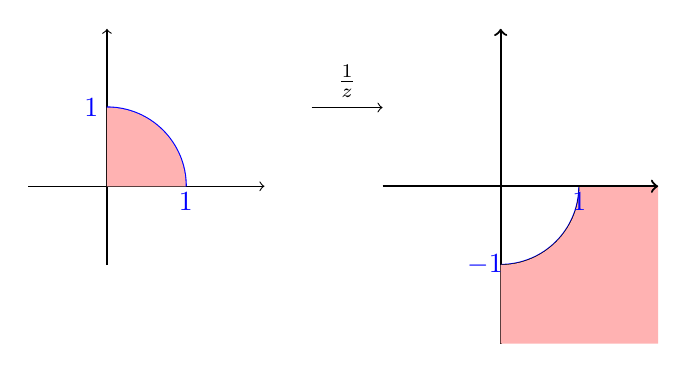
\begin{tikzpicture}

% First coordinate system (z-plane)
\begin{scope}
    \draw[->] (-1,0) -- (2,0);
    \draw[->] (0,-1) -- (0,2);

    \draw[blue, thick] (0,0) + (1,0) arc (0:90:1);

    \fill[red!30] (0,0) -- (1,0) arc (0:90:1) -- cycle;

    \node[blue] at (1, -0.2) {$1$};
    \node[blue] at (-0.2, 1) {$1$};
\end{scope}

% Transformation arrow
\draw[->] (2.6,1) -- (3.5,1) node[midway, above] {$\frac{1}{z}$};

% Second coordinate system (w-plane)
\begin{scope}[shift={(5,0)}]
   
    \draw[->, thick] (0,-2) -- (0,2);

    \draw[blue, thick] (0,0) + (1,0) arc (0:-90:1);

    \draw (0,0) -- (1,0) arc (0:-90:1) -- cycle;

    \fill[red!30] (1,0) arc (0:-90:1) -- (0,-2) -- (2,-2) -- (2,0) -- cycle;

    \node[blue] at (1, -0.2) {$1$};
    \node[blue] at (-0.2, -1) {$-1$};
	 \draw[->, thick] (-1.5,0) -- (2,0);
    % Approximate the shaded square
  %  \fill[black!80] (0.5,0.5) -- (-0.5,0.5) -- (-0.5,-0.5) -- (0.5,-0.5) -- cycle;
\end{scope}

\end{tikzpicture}

\end{document}